\documentclass{article}

\usepackage[a4paper, left=1.5cm, right=1.5cm, top=2cm, bottom=2cm]{geometry}
\usepackage{../../../components/mathtex}
\usepackage{pgfplots}
\pgfplotsset{compat=1.18}
\usepackage{hyperref}
\usepackage{fancyhdr}
\usepackage{ccicons}
\usepackage{caption}
\usepackage{subcaption}
\usepackage{tikz}
\usetikzlibrary{shapes, arrows.meta, positioning, calc}

% Configuration des en-têtes et pieds de page
\pagestyle{fancy}
\fancyhf{}

\fancyhead[L]{DL3 Math-Info SY5}
\fancyhead[C]{Systèmes d'Exploitation 5}
\fancyhead[R]{2026-2027}

\fancyfoot[L]{Ewen Rodrigues de Oliveira\\\ccbyncsa}
\fancyfoot[R]{\thepage}

\begin{document}

\docTitle{Chapitre 1 : Introduction aux Systèmes d'Exploitation et Entrées/Sorties}

% ==========================================
% SECTION 1 : INTRODUCTION AUX SYSTÈMES D'EXPLOITATION
% ==========================================
\section{Introduction aux Systèmes d'Exploitation}

\subsection{Rôle du système d'exploitation}

\definition{
    Un \textbf{Système d'Exploitation} (SE) est une couche logicielle qui fait l'interface entre le matériel (processeur, mémoire, périphériques) et les applications ou l'utilisateur. Il fournit le bon niveau d'abstraction et gère les ressources de façon équitable et sécurisée.
}

\remark{
    Pour garantir la sécurité et l'équité, les processeurs modernes possèdent au moins deux modes de fonctionnement :
    \begin{itemize}
        \item \textbf{Mode Utilisateur (User mode) :} Mode bridé où seules les instructions inoffensives sont exécutées.
        \item \textbf{Mode Noyau (Kernel mode) :} Mode privilégié où toutes les instructions et tous les accès matériels sont autorisés.
    \end{itemize}
    La transition entre le mode utilisateur et le mode noyau s'effectue via un \textbf{appel système} (\textit{syscall}).
}

\subsection{Espace d'adressage et états d'un processus}

\definition{
    Un \textbf{processus} est l'instance dynamique d'un programme en cours d'exécution. Il possède un espace d'adressage propre divisé en :
    \begin{itemize}
        \item \textbf{Code (Text) :} Instructions exécutables du programme.
        \item \textbf{Données statiques (Data/BSS) :} Variables globales et statiques.
        \item \textbf{Tas (Heap) :} Zone d'allocation dynamique (\texttt{malloc}).
        \item \textbf{Pile (Stack) :} Zone de stockage des variables locales et contextes d'appel.
    \end{itemize}
}

\begin{center}
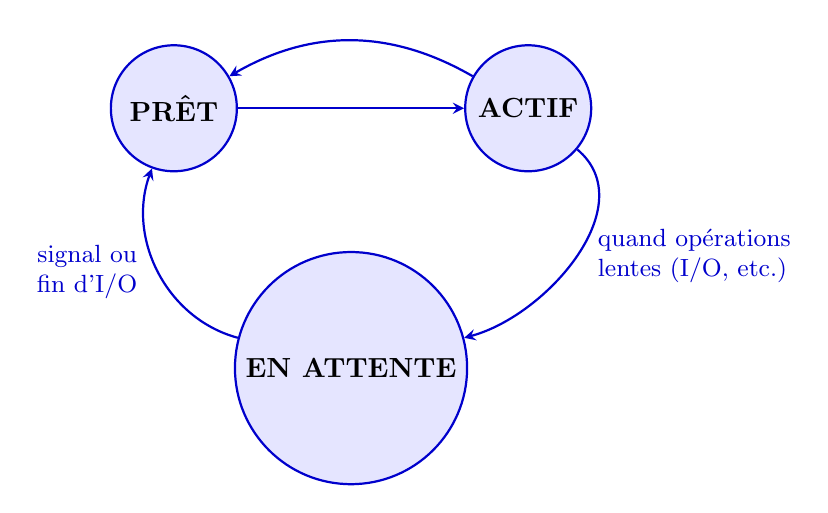
\begin{tikzpicture}[
    state/.style={circle, draw=blue!80!black, thick, minimum size=1.6cm, align=center, font=\bfseries},
    >=stealth
]
    % Nœuds principaux
    \node[state, fill=blue!10] (pret) at (0, 2.5) {PRÊT};
    \node[state, fill=blue!10] (actif) at (4.5, 2.5) {ACTIF};
    \node[state, fill=blue!10] (attente) at (2.25, -0.8) {EN ATTENTE};

    % Flèche PRÊT -> ACTIF
    \draw[->, thick, blue!80!black] (pret) -- (actif);

    % Flèche ACTIF -> PRÊT (retour)
    \draw[->, thick, blue!80!black] (actif) to[out=150, in=30] (pret);

    % Flèche ACTIF -> EN ATTENTE
    \draw[->, thick, blue!80!black] (actif) to[out=-40, in=15] node[midway, right=4pt, align=left, font=\small] {quand opérations\\lentes (I/O, etc.)} (attente);

    % Flèche EN ATTENTE -> PRÊT
    \draw[->, thick, blue!80!black] (attente) to[out=165, in=-110] node[midway, left=4pt, align=right, font=\small] {signal ou\\fin d'I/O} (pret);

\end{tikzpicture}
\captionof{figure}{Diagramme des états d'un processus}
\end{center}

\subsection{Hiérarchie des mémoires}

\theorem{Principe}{Hiérarchie de stockage}{false}{
    Les composants de stockage présentent des compromis opposés entre la vitesse d'accès, la capacité et le coût :
    \begin{enumerate}
        \item \textbf{Registres} ($\sim 0.5$ ns, très faibles capacités).
        \item \textbf{Caches} ($\sim 2$ ns).
        \item \textbf{Mémoire RAM} ($\sim 10$ ns) — volatile.
        \item \textbf{Stockage secondaire SSD / HDD} ($0.1$ ms à $10$ ms) — non volatile.
        \item \textbf{Bandes magnétiques} ($\sim 100$ s) — archivage.
    \end{enumerate}
}

% ==========================================
% SECTION 2 : GESTION DES ENTRÉES/SORTIES ET FICHIERS
% ==========================================
\section{Gestion des Entrées/Sorties et Fichiers}

\subsection{Descripteurs et tables de fichiers}

\definition{
    Un \textbf{descripteur de fichier} (\textit{file descriptor} ou \texttt{fd}) est un entier positif renvoyé par un appel système (comme \texttt{open}) qui sert d'index à un processus pour accéder à un fichier.
}

\remark{
    Tout processus hérite par défaut de 3 descripteurs ouverts :
    \begin{itemize}
        \item \texttt{0} : Entrée standard (\texttt{STDIN\_FILENO}).
        \item \texttt{1} : Sortie standard (\texttt{STDOUT\_FILENO}).
        \item \texttt{2} : Sortie d'erreur standard (\texttt{STDERR\_FILENO}).
    \end{itemize}
}

\begin{center}
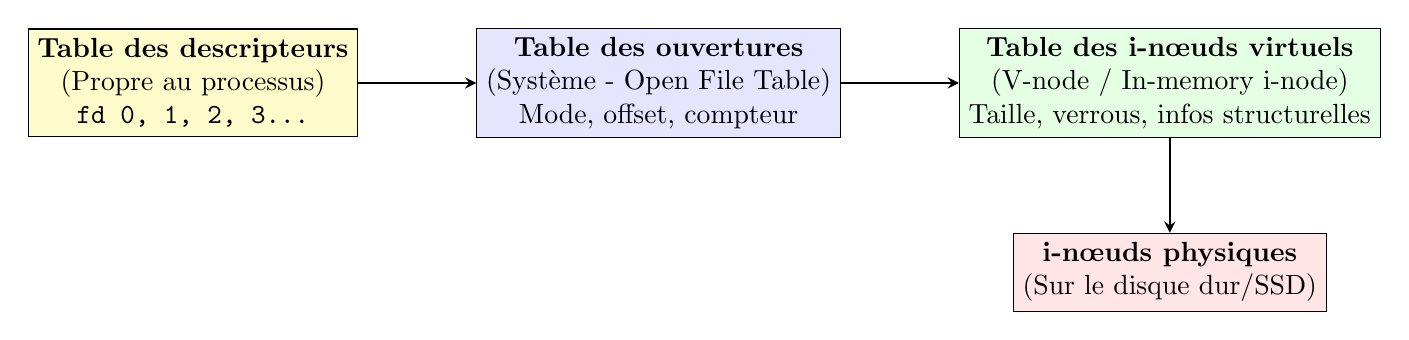
\begin{tikzpicture}[node distance=1.5cm, >=stealth, block/.style={draw, rectangle, minimum height=0.8cm, align=center}]

    % Processus
    \node[block, fill=yellow!20] (fdtable) {\textbf{Table des descripteurs}\\(Propre au processus)\\ \texttt{fd 0, 1, 2, 3...}};
    
    % Table des ouvertures
    \node[block, fill=blue!10, right=1.5cm of fdtable] (openfile) {\textbf{Table des ouvertures}\\(Système - Open File Table)\\Mode, offset, compteur};
    
    % Table des i-nœuds virtuels
    \node[block, fill=green!10, right=1.5cm of openfile] (vnode) {\textbf{Table des i-nœuds virtuels}\\(V-node / In-memory i-node)\\Taille, verrous, infos structurelles};
    
    % Disque dur
    \node[block, fill=red!10, below=1.2cm of vnode] (inode) {\textbf{i-nœuds physiques}\\(Sur le disque dur/SSD)};

    % Liens
    \draw[->, thick] (fdtable) -- (openfile);
    \draw[->, thick] (openfile) -- (vnode);
    \draw[->, thick] (vnode) -- (inode);

\end{tikzpicture}
\captionof{figure}{Indirections lors de l'accès à un fichier}
\end{center}

\subsection{Appels système fondamentaux pour les I/O}

\method{Manipuler un fichier via les appels système}{
    \begin{enumerate}
        \item \textbf{Ouverture (\texttt{open}) :}
        
        \texttt{int open(const char *pathname, int flags, mode\_t mode);}
        
        Les flags obligatoires sont \texttt{O\_RDONLY}, \texttt{O\_WRONLY}, ou \texttt{O\_RDWR}. On peut les combiner avec \texttt{O\_CREAT}, \texttt{O\_TRUNC}, \texttt{O\_APPEND}, \texttt{O\_EXCL} via un \texttt{OR} bit-à-bit (\texttt{|}).

        \item \textbf{Lecture (\texttt{read}) :}
        
        \texttt{ssize\_t read(int fd, void *buf, size\_t count);}
        
        Lit au plus \texttt{count} octets et les place dans \texttt{buf}. Renvoie le nombre d'octets lus, \texttt{0} à la fin du fichier, ou \texttt{-1} en cas d'erreur.

        \item \textbf{Écriture (\texttt{write}) :}
        
        \texttt{ssize\_t write(int fd, const void *buf, size\_t count);}
        
        Écrit \texttt{count} octets depuis \texttt{buf} dans le fichier.

        \item \textbf{Positionnement (\texttt{lseek}) :}
        
        \texttt{off\_t lseek(int fd, off\_t offset, int whence);}
        
        Modifie la position de la tête de lecture/écriture selon \texttt{whence} (\texttt{SEEK\_SET}, \texttt{SEEK\_CUR}, \texttt{SEEK\_END}).

        \item \textbf{Fermeture (\texttt{close}) :}
        
        \texttt{int close(int fd);}
        
        Libère le descripteur et met à jour les compteurs dans les tables système.
    \end{enumerate}
}

\subsection{Surcouche \texttt{FILE*} de la bibliothèque standard}

\remark{
    La bibliothèque standard C (\texttt{stdio.h}) propose des fonctions de plus haut niveau manipulant des pointeurs \texttt{FILE*}.
    Un objet \texttt{FILE} encapsule un descripteur de fichier et y ajoute un \textbf{tampon mémoire (buffer)} pour réduire le nombre d'appels système.
}

\attention{
    Le buffer d'un flot \texttt{FILE*} est vidé (\textit{flushed}) automatiquement dans les cas suivants :
    \begin{itemize}
        \item Quand le tampon est plein.
        \item Lors d'un appel explicite à \texttt{fflush(stream)}.
        \item À la fermeture avec \texttt{fclose(stream)}.
        \item À la fin normale du processus via \texttt{exit} (mais \textbf{pas} lors d'un arrêt brutal comme un \texttt{SIGKILL} ou un crash).
        \item Pour les sorties sur terminal, à chaque saut de ligne (\texttt{'\textbackslash n'}).
    \end{itemize}
}

\subsection{Notion d'atomicité}

\definition{
    Une opération est dite \textbf{atomique} si elle s'exécute en une seule étape ininterrompue par le système d'exploitation.
}

\example{
    L'ouverture avec \texttt{O\_CREAT | O\_EXCL} garantit que la vérification de l'existence et la création du fichier se font de façon atomique. De même, l'ouverture en mode \texttt{O\_APPEND} garantit que le repositionnement en fin de fichier et l'écriture s'effectuent atomiquement.
}

\end{document}